\documentclass[a4paper,12pt,headsepline]{scrartcl}
\usepackage{tikz}
\usepackage{tikz-qtree}
\usepackage{fix-cm}
\begin{document}
\begin{center} 
\begin{tabular}{l}$B\rightarrow S C~~$\\ 
$C\rightarrow b~|~a~~$\\ 
$S\rightarrow C C~|~S C~~$\\ 
\end{tabular} 
\end{center}
\begin{center}
\resizebox{\linewidth}{!}{
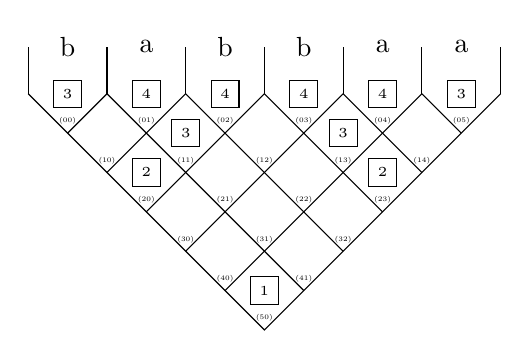
\begin{tikzpicture}[baseline]
\newcommand{\myfontvars}[1]{
\fontsize{4.9}{12}\selectfont{#1}
}\newcommand{\myfontnumbering}[1]{
\fontsize{2.5}{12}\selectfont{#1}
}%Outer hull
%Tip of the pyramid
\coordinate (tip) at (3.0,-3.0);
\foreach \i in {0,...,6} {
 	\coordinate (\i) at (\i,0);
}
%Draw the left and right line of the pyramid pointing downwards
\draw (0) -- (tip) -- (6);
%Grid lines direction down-left to top-right
\coordinate (dl1) at (0.5,-0.5);
\coordinate (dl2) at (1.0,-1.0);
\coordinate (dl3) at (1.5,-1.5);
\coordinate (dl4) at (2.0,-2.0);
\coordinate (dl5) at (2.5,-2.5);
\draw (dl1) -- (1,0);
\draw (dl2) -- (2,0);
\draw (dl3) -- (3,0);
\draw (dl4) -- (4,0);
\draw (dl5) -- (5,0);
%Grid lines direction down-right to top-left
\coordinate (dr1) at (3.5,-2.5);
\coordinate (dr2) at (4.0,-2.0);
\coordinate (dr3) at (4.5,-1.5);
\coordinate (dr4) at (5.0,-1.0);
\coordinate (dr5) at (5.5,-0.5);
\draw (dr1) -- (1,0);
\draw (dr2) -- (2,0);
\draw (dr3) -- (3,0);
\draw (dr4) -- (4,0);
\draw (dr5) -- (5,0);
%Small lines at the top
\coordinate (top0) at (0.0,0.0);
\coordinate (top1) at (1.0,0.0);
\coordinate (top2) at (2.0,0.0);
\coordinate (top3) at (3.0,0.0);
\coordinate (top4) at (4.0,0.0);
\coordinate (top5) at (5.0,0.0);
\coordinate (top6) at (6.0,0.0);
\coordinate (topUpper0) at (0.0,0.6);
\coordinate (topUpper1) at (1.0,0.6);
\coordinate (topUpper2) at (2.0,0.6);
\coordinate (topUpper3) at (3.0,0.6);
\coordinate (topUpper4) at (4.0,0.6);
\coordinate (topUpper5) at (5.0,0.6);
\coordinate (topUpper6) at (6.0,0.6);
\draw (top0) -- (topUpper0);
\draw (top1) -- (topUpper1);
\draw (top2) -- (topUpper2);
\draw (top3) -- (topUpper3);
\draw (top4) -- (topUpper4);
\draw (top5) -- (topUpper5);
\draw (top6) -- (topUpper6);
%The string
\coordinate (w0) at (0.5,0.6);
\coordinate (w1) at (1.5,0.6);
\coordinate (w2) at (2.5,0.6);
\coordinate (w3) at (3.5,0.6);
\coordinate (w4) at (4.5,0.6);
\coordinate (w5) at (5.5,0.6);
\node [] at (w0) {b};
\node [] at (w1) {a};
\node [] at (w2) {b};
\node [] at (w3) {b};
\node [] at (w4) {a};
\node [] at (w5) {a};
% Variables in the cells
%cells00
\coordinate (center00) at (0.5,0.0);
\node [below=0.18cm] at (center00) {\myfontnumbering{$(00)$}};
\node [] at (center00) [minimum height=0.25cm,minimum width=0.25cm,draw] {\tiny{3}};
%cells01
\coordinate (center01) at (1.5,0.0);
\node [below=0.18cm] at (center01) {\myfontnumbering{$(01)$}};
\node [] at (center01) [minimum height=0.25cm,minimum width=0.25cm,draw] {\tiny{4}};
%cells02
\coordinate (center02) at (2.5,0.0);
\node [below=0.18cm] at (center02) {\myfontnumbering{$(02)$}};
\node [] at (center02) [minimum height=0.25cm,minimum width=0.25cm,draw] {\tiny{4}};
%cells03
\coordinate (center03) at (3.5,0.0);
\node [below=0.18cm] at (center03) {\myfontnumbering{$(03)$}};
\node [] at (center03) [minimum height=0.25cm,minimum width=0.25cm,draw] {\tiny{4}};
%cells04
\coordinate (center04) at (4.5,0.0);
\node [below=0.18cm] at (center04) {\myfontnumbering{$(04)$}};
\node [] at (center04) [minimum height=0.25cm,minimum width=0.25cm,draw] {\tiny{4}};
%cells05
\coordinate (center05) at (5.5,0.0);
\node [below=0.18cm] at (center05) {\myfontnumbering{$(05)$}};
\node [] at (center05) [minimum height=0.25cm,minimum width=0.25cm,draw] {\tiny{3}};
%cells10
\coordinate (center10) at (1.0,-0.5);
\node [below=0.18cm] at (center10) {\myfontnumbering{$(10)$}};
%cells11
\coordinate (center11) at (2.0,-0.5);
\node [below=0.18cm] at (center11) {\myfontnumbering{$(11)$}};
\node [] at (center11) [minimum height=0.25cm,minimum width=0.25cm,draw] {\tiny{3}};
%cells12
\coordinate (center12) at (3.0,-0.5);
\node [below=0.18cm] at (center12) {\myfontnumbering{$(12)$}};
%cells13
\coordinate (center13) at (4.0,-0.5);
\node [below=0.18cm] at (center13) {\myfontnumbering{$(13)$}};
\node [] at (center13) [minimum height=0.25cm,minimum width=0.25cm,draw] {\tiny{3}};
%cells14
\coordinate (center14) at (5.0,-0.5);
\node [below=0.18cm] at (center14) {\myfontnumbering{$(14)$}};
%cells20
\coordinate (center20) at (1.5,-1.0);
\node [below=0.18cm] at (center20) {\myfontnumbering{$(20)$}};
\node [] at (center20) [minimum height=0.25cm,minimum width=0.25cm,draw] {\tiny{2}};
%cells21
\coordinate (center21) at (2.5,-1.0);
\node [below=0.18cm] at (center21) {\myfontnumbering{$(21)$}};
%cells22
\coordinate (center22) at (3.5,-1.0);
\node [below=0.18cm] at (center22) {\myfontnumbering{$(22)$}};
%cells23
\coordinate (center23) at (4.5,-1.0);
\node [below=0.18cm] at (center23) {\myfontnumbering{$(23)$}};
\node [] at (center23) [minimum height=0.25cm,minimum width=0.25cm,draw] {\tiny{2}};
%cells30
\coordinate (center30) at (2.0,-1.5);
\node [below=0.18cm] at (center30) {\myfontnumbering{$(30)$}};
%cells31
\coordinate (center31) at (3.0,-1.5);
\node [below=0.18cm] at (center31) {\myfontnumbering{$(31)$}};
%cells32
\coordinate (center32) at (4.0,-1.5);
\node [below=0.18cm] at (center32) {\myfontnumbering{$(32)$}};
%cells40
\coordinate (center40) at (2.5,-2.0);
\node [below=0.18cm] at (center40) {\myfontnumbering{$(40)$}};
%cells41
\coordinate (center41) at (3.5,-2.0);
\node [below=0.18cm] at (center41) {\myfontnumbering{$(41)$}};
%cells50
\coordinate (center50) at (3.0,-2.5);
\node [below=0.18cm] at (center50) {\myfontnumbering{$(50)$}};
\node [] at (center50) [minimum height=0.25cm,minimum width=0.25cm,draw] {\tiny{1}};
\end{tikzpicture}
}
\end{center}
\begin{center}
\resizebox{\linewidth}{!}{
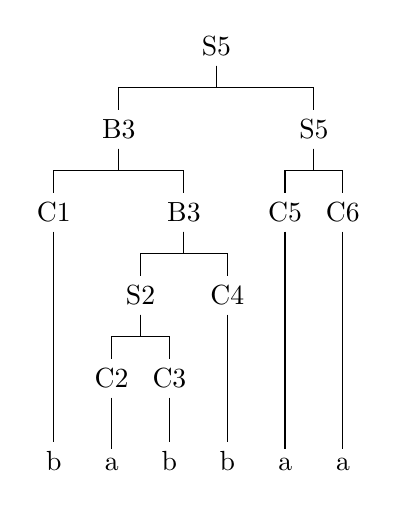
\begin{tikzpicture}[baseline]
		\tikzset{frontier/.style={distance from root=150pt}} %height of tree times 30pt
		\tikzset{edge from parent/.style= {
				draw,
				edge from parent path={(\tikzparentnode.south)	-- +(0,-8pt)-| (\tikzchildnode)}
			}
		}
		\Tree
[.S5
[.B3
[.C1 b ]
[.B3
[.S2
[.C2 a ]
[.C3 b ]
]
[.C4 b ]
]
]
[.S5
[.C5 a ]
[.C6 a ]
]
]
\end{tikzpicture}
}
\end{center}
\end{document}
